\documentclass[../main/main.tex]{subfiles}
\graphicspath{{./figures/}}

\makeatletter
\renewcommand{\@chapapp}{Travaux pratiques -- TP}
\makeatother

% \toggletrue{student}
% \toggletrue{corrige}
% \renewcommand{\mycol}{black}
\renewcommand{\mycol}{gray}

\begin{document}
\setcounter{chapter}{19}

\settype{enon}
\settype{solu_prof}
\settype{solu_stud}

\chapter{\cswitch{%
	  Correction du TP
  }{%
	  \'Etude des oscillations forc\'ees d'un oscillateur m\'ecanique amorti
  }
 }

\enonce{%
	\begin{prgm}
		\begin{tcb}*(ror)"how"{Savoir-faire}
			\begin{itemize}
				\item Mettre en œuvre un accéléromètre, par exemple avec l’aide d’un
				      microcontrôleur.
				\item Effectuer des représentations graphiques à partir de données.
				\item Mener des calculs analytiques ou à l’aide d’un langage de
				      programmation, effectuer des applications numériques.
				\item Confronter les résultats d’un modèle à des résultats
				      expérimentaux
			\end{itemize}
		\end{tcb}
	\end{prgm}
	\vspace{-10pt}

	\section{Objectifs}

	\begin{itemize}
		\item Utiliser un microcontrôleur Arduino afin de mettre en œuvre un
		      accéléromètre.
		\item Tracer l'allure de la courbe de résonance en vitesse et en position.
		\item Vérifier les principales caractéristiques des oscillations mécaniques
		      forcées.
		\item Déterminer le facteur de qualité du montage.
		\item Développer une approche de recherche vis-a-vis de la détermination
		      de paramètres physiques \textit{via} une minimisation en
		      \texttt{Python}.
	\end{itemize}

	\section{S'approprier~: montage expérimental}

	\begin{minipage}{0.60\linewidth}
		Une masse $m$, assimilée à un point matériel $M$, est suspendue entre deux
		ressorts dont l'un d'eux -- celui du haut -- est relié à un pot vibrant
		permettant d'induire un mouvement linéaire quasi sinusoïdal d'amplitude
		constante mais de fréquence réglable. Le déplacement du système vibrant dans
		l'air est à l'origine d'un amortissement fluide modélisé par une force du
		type~:
		\[
			\Ff = -\a\vf
		\]
		Un accéléromètre est attaché directement à la masse en translation verticale
		afin de suivre son déplacement au cours du temps.
	\end{minipage}
	\hfill
	\begin{minipage}{0.40\linewidth}
		\begin{center}
			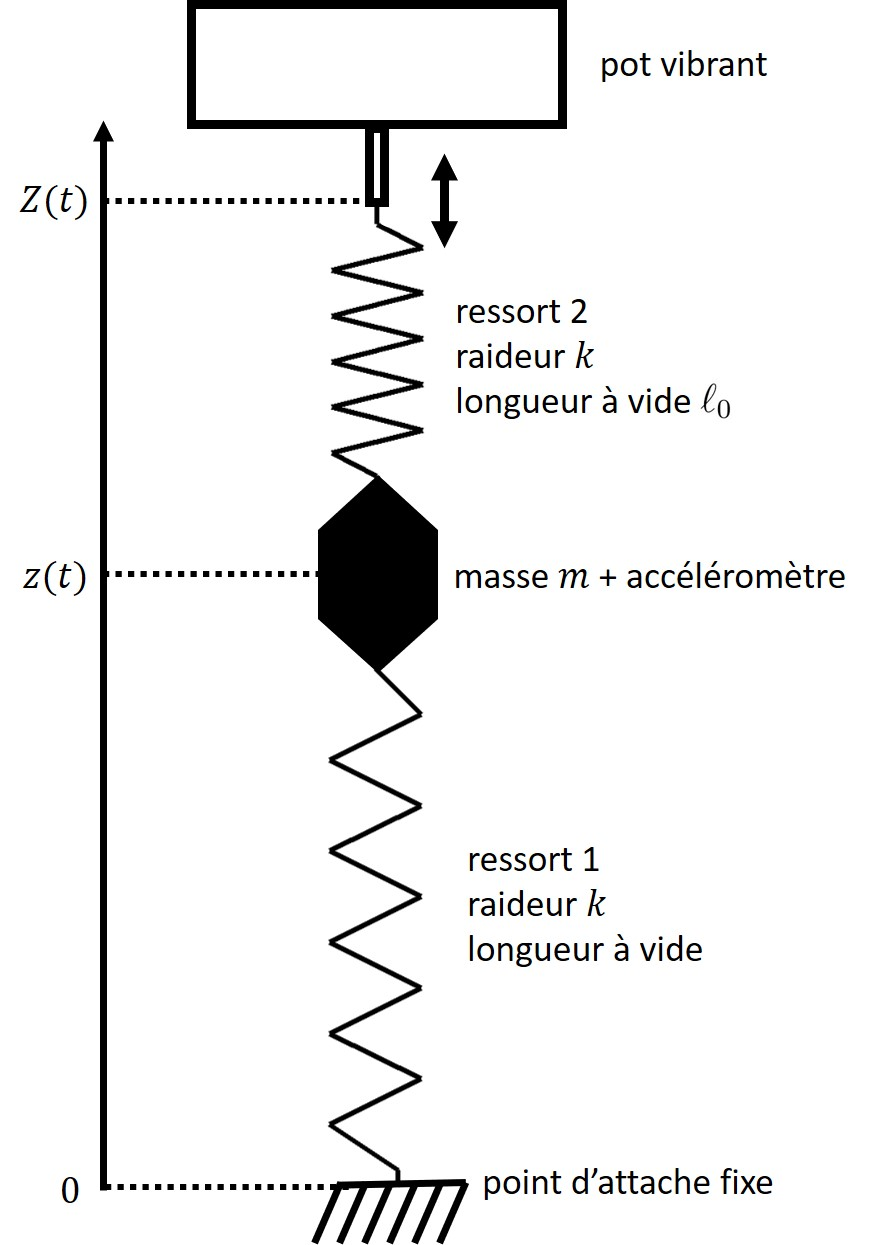
\includegraphics[height=7cm]{arduino_schema}
		\end{center}
	\end{minipage}
}

\section{Analyser}

\enonce{%
	On repère la position de la masse $m$ grâce à son abscisse $z(t)$ sur l'axe
	$(\Or z)$ dont l'origine O est au point d'attache fixe du ressort $(1)$. Les
	deux ressorts ont une longueur à vide $\ell_0$ et sont de raideur $k$. Le
	ressort du dessus peut bouger avec le vibreur, et son point d'attache est
	repéré par l'abscisse $Z(t)$.
}

\subsection{À excitation nulle}

\enonce{%
	À excitation nulle, on suppose que $Z(t) = h$, une constante.
}

\setlist[blocQR,1]{leftmargin=10pt, label=\clenumi}
\QR[5]{%
	Montrer que la longueur du ressort $(1)$ à l'équilibre est
	$\DS z\ind{eq} = \frac{h}{2} - \frac{mg}{2k}$
}{%
	\noindent
	\begin{minipage}[t]{.60\linewidth}
		\begin{itemize}
			\bitem{Système}~: \{masse\} assimilée à un point matériel M de masse $m$.
			\bitem{Référentiel}~: terrestre supposé galiléen.
			\bitem{Repère}~: $(\Or, \uz)$ vertical ascendant.
			\bitem{Repérage}~:
			\[
				\left\{
				\begin{array}{rl}
					\OM & = z(t)\uz
					\\
					\vf & = \zp(t)\uz
					\\
					\af & = \zpp(t)\uz
				\end{array}
				\right.
			\]
			De plus, à excitation nulle on trouve
			\[
				\ell_1(t) = z(t)
				\qet
				\ell_2(t) = Z(t) - z(t) = h - z(t)
			\]
			\bitem{BdF}~:
			\begin{itemize}
				\item $\Pf = -mg\uz$
				\item
				      $\Ff_{r,1} =
					      -k \left( \ell_1(t) - \ell_0 \right)\uz =
					      - k \left( z(t) - \ell_0 \right)\uz$
				\item
				      $\Ff_{r,2} =
					      +k \left( \ell_2(t) - \ell_0 \right)\uz =
					      +k \left( h - z(t) - \ell_0 \right)\uz$
				\item $\Ff = -\alpha\vf = -\alpha \zp(t)\uz$
			\end{itemize}
		\end{itemize}
	\end{minipage}
	\hfill
	\begin{minipage}[t]{.45\linewidth}
		\vspace{0pt}
		\begin{center}
			\includegraphics[width=\linewidth]{arduino_corr}
		\end{center}
	\end{minipage}
	\begin{itemize}
		\bitem{PFD}~: à l'équilibre,
		\begin{DispWithArrows*}
			\af = \of &= \sum_i \Ff_i
			\Arrow{On projette}
			\\\Lra
			0 &=
			-mg
			-k \left( z\ind{eq} - \cancel{\ell_0} \right)
			+ k \left( h - z\ind{eq} - \cancel{\ell_0} \right)
			\underbracket[1pt]{-\alpha \zp\ind{eq}}_{=0}
			\Arrow{On isole}
			\\\Lra
			2k z\ind{eq} &= kh - mg
			\\\Lra
			\Aboxed{z\ind{eq} &= \frac{h}{2} - \frac{mg}{2k}}
			\qed
		\end{DispWithArrows*}
	\end{itemize}
}

\QR[3]{%
On pose $\ell(t) = z(t)-z\ind{eq}$. Montrer que l'équation différentielle du
mouvement de la masse $m$ peut se mettre sous la forme canonique~:
\[
	\ddot{\ell} + \frac{\w_0}{Q} \dot{\ell} + {\w_0}^2 \ell = 0
\]
Identifier $\w_0$ et $Q$, rappeler leur nom et leur unité.
}{%
On reprend le PFD précédent mais $\forall t$, en remarquant que $\lpp = \zpp$
et $\lp = \zp$~:
\begin{DispWithArrows*}[]
	m\af &= \sum_i \Ff_i
	\CArrow{$\cdot \uz$}
	\\\Lra
	m\zpp(t) &=
	-mg
	- k \left( z(t) - \cancel{\ell_0} \right)
	+ k \left( h - z(t) - \cancel{\ell_0} \right)
	- \alpha \zp(t)
	\CArrow{$\mdiv m$}
	\\\Lra
	\zpp(t) +
	\frac{\alpha}{m} \zp(t) +
	\xunderbracket{\frac{2k}{m}}_{=\w_0{}^2} z(t) &=
	\xunderbracket{-g +\frac{k}{m}h}_{= \w_0{}^2 z\ind{eq}}
	\\\Lra
	\zpp(t) +
	\frac{\alpha}{m} \zp(t) +
	\w_0{}^2 \left( z(t) - z\ind{eq} \right) &= 0
	\\\Lra
	\Aboxed{\lpp + \frac{\w_0}{Q} + \w_0{}^2 \ell &= 0}
	\qed
\end{DispWithArrows*}
On trouve ainsi $\w_0$ la pulsation propre et $Q$ le facteur de qualité tels
que~:
\[
	\w_0{}^2 = \frac{2k}{m} \Lra \boxed{\w_0 = \sqrt{\frac{2k}{m}}} \quad
	[\si{rad.s^{-1}}]
	\qet
	\frac{\w_0}{Q} = \frac{\alpha}{m} \Lra \boxed{Q = \frac{\sqrt{2km}}{\alpha}}
	\quad \text{sans unité}
\]
}

\QR[1]{%
	Quel est le ressort équivalent aux deux ressorts~?
}{%
	Par identification avec le résultat pour un unique ressort, on trouve
	\[
		\boxed{k' = 2k} \qet \boxed{\ell_0' = \frac{h}{2}}
	\]
}

\subsection{En régime sinusoïdal forcé}

\enonce{%
	\begin{isd}
		On se place en régime sinusoïdal forcé, et on suppose que le point d'attache
		haut du ressort (2) suit un mouvement sinusoïdal autour de sa position
		d'équilibre $h$~:
		\[
			Z(t) = h + \alpha \cos(\w t)
		\]
		\tcblower
		Ainsi, le mouvement de la masse est lui aussi sinusoïdal, de même fréquence
		que le forçage~:
		\[\ell(t) = L\cos(\wt+\f)\]
	\end{isd}
}

\QR[2]{%
	Rappeler l'allure des courbes de résonance (amplitude des oscillations
	en fonction de la fréquence) en position ($\ell(t)$) et en vitesse ($v_z
		= \lp(t)$) pour un tel système mécanique. À quel type de filtre
	correspond chaque courbe~?
}{%
	On trouve les courbes suivantes pour la tension/élongation et
	l'intensité/vitesse (par analogie au RLC série)~:
	\smallbreak
	\begin{isd}
		\tcbsubtitle{\fatbox{\textbf{Élongation}}}
		\begin{center}
			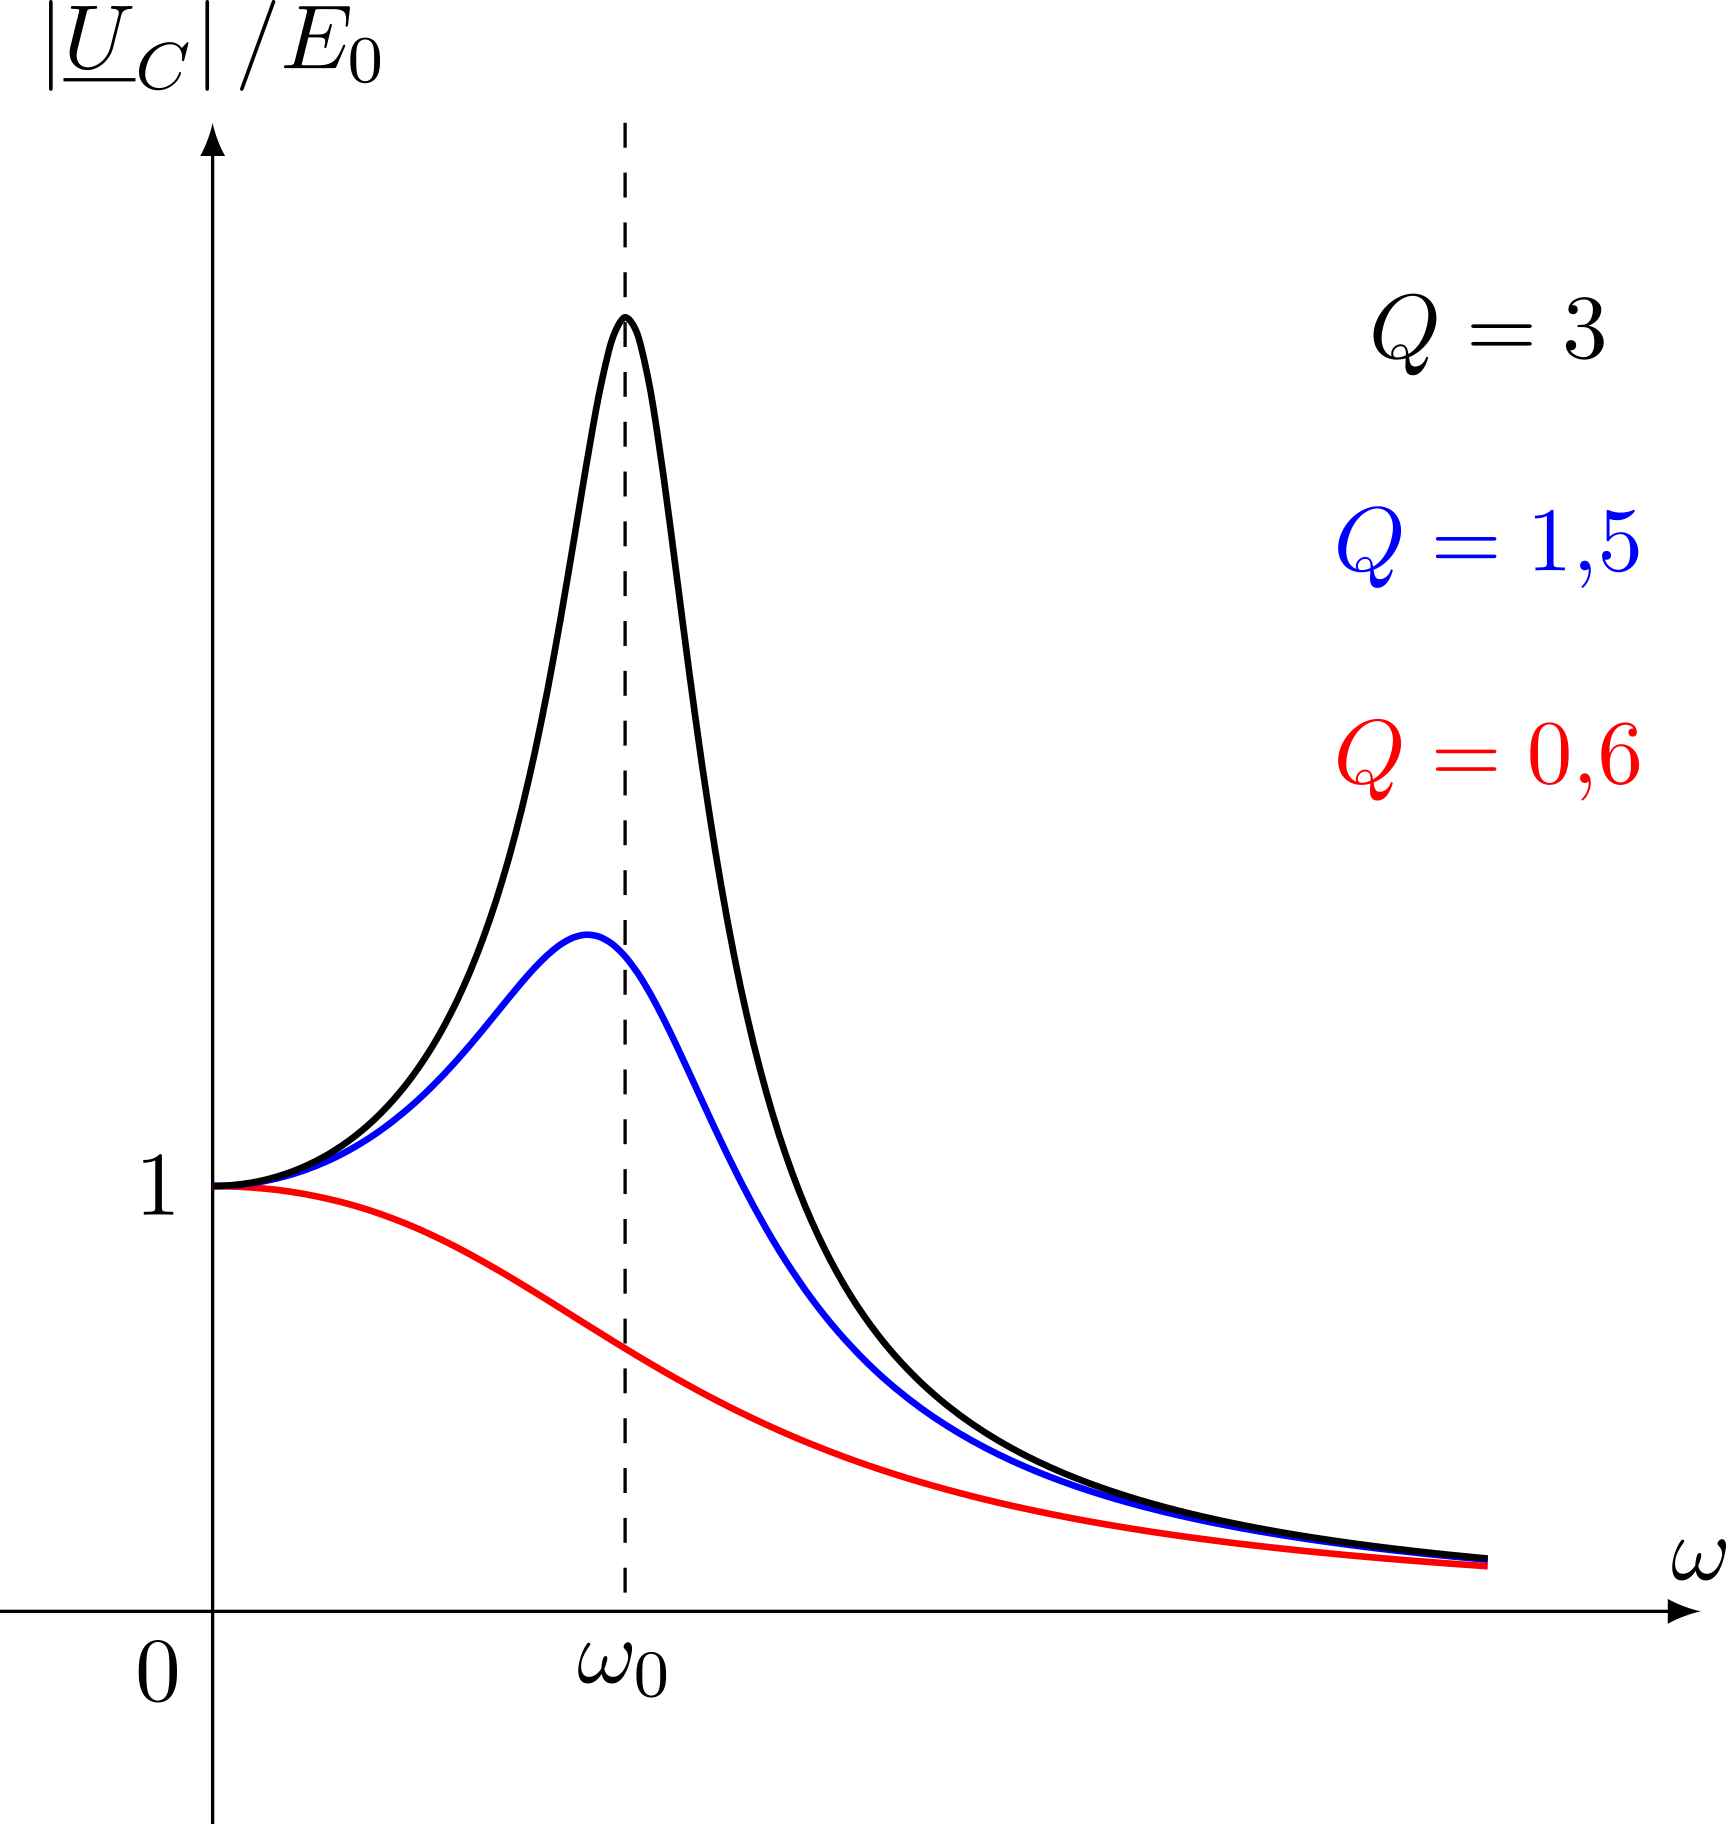
\includegraphics[width=.7\linewidth]{rlc_u-amp}
			\captionsetup{justification=centering}
			\captionof{figure}{Résonance en élongation\\Filtre passe-bas}
		\end{center}
		\tcblower
		\tcbsubtitle{\fatbox{\textbf{Vitesse}}}
		\begin{center}
			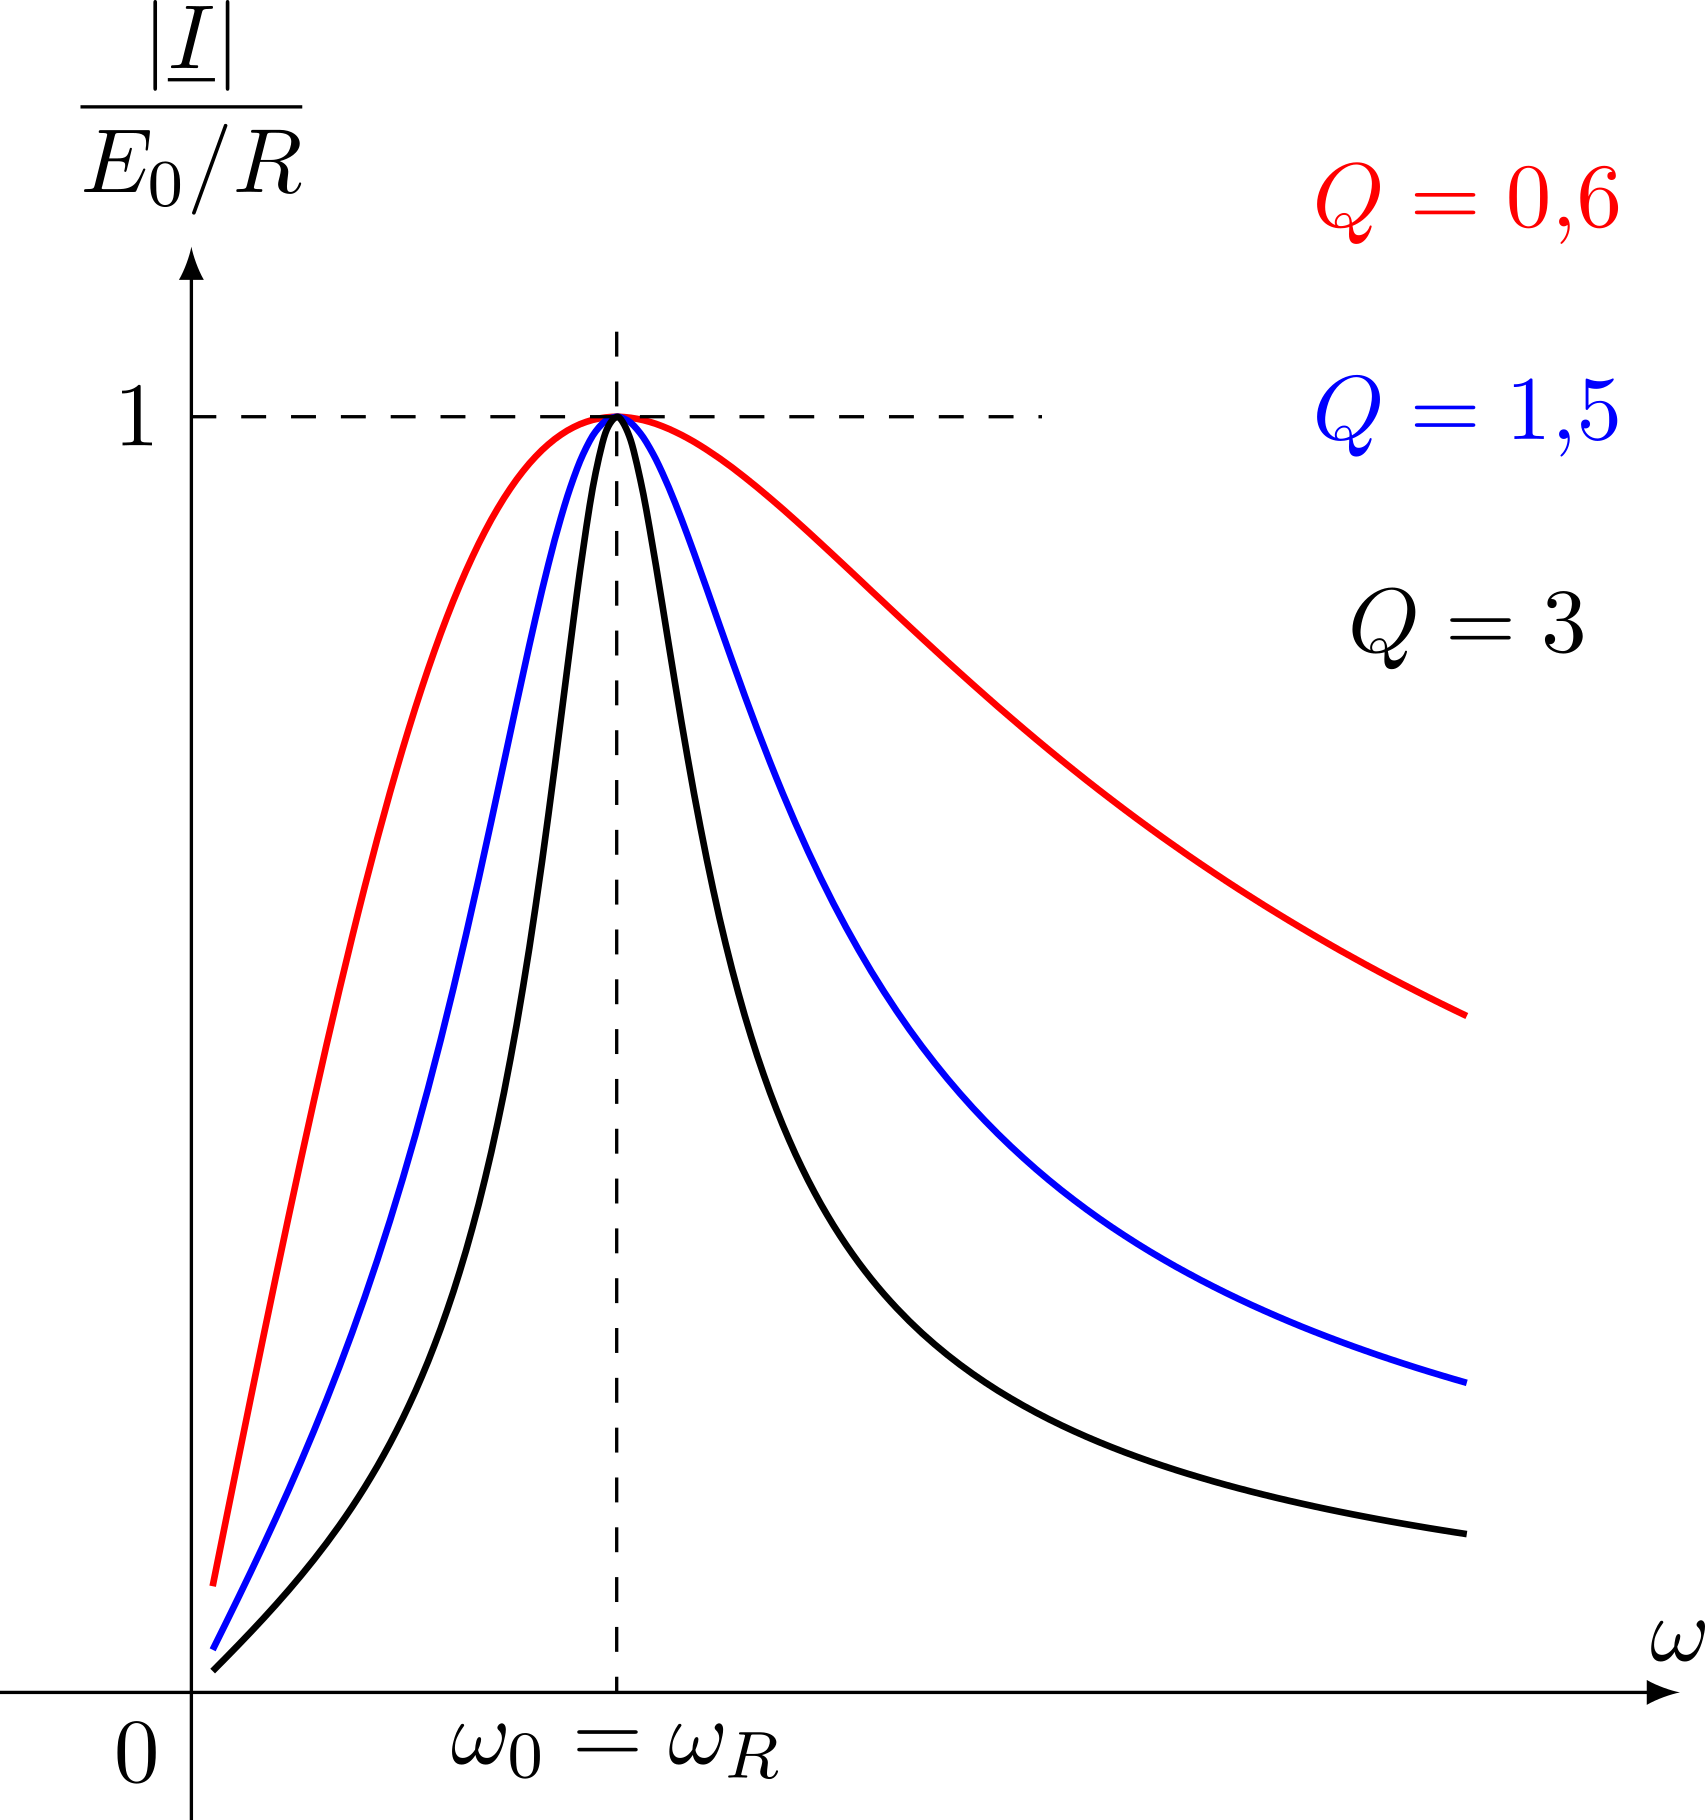
\includegraphics[width=.7\linewidth]{rlc_i-amp}
			\captionsetup{justification=centering}
			\captionof{figure}{Résonance en vitesse\\Filtre passe-bande}
		\end{center}
	\end{isd}
}

\QR[1]{%
	Exprimer $v_z = \lp(t)$ et $a_z = \lpp(t)$, puis les
	amplitudes $V$ et $A$ de leurs oscillations en fonction de $L$ et $\w$.
}{%
	En RSF, on aura $\ell(t) = L \cos(\wt + \f)$, d'où
	\begin{align*}
		v_z(t) = -L\w \sin(\wt + \f)   & \Ra \boxed{V = L\w}
		\\
		a_z(t) = -L\w^2 \cos(\wt + \f) & \Ra \boxed{A = L\w^2}
	\end{align*}
}

\QR[1]{%
	Quelle relation relie la bande passante et le facteur de qualité lors
	de la résonance en vitesse~?
}{%
	C'est l'acuité de la résonance~:
	\[
		\boxed{\Delta\w = \frac{\w_0}{Q}} \Lra \boxed{Q = \frac{\w_0}{\Delta\w}}
	\]
}

\enonce{%
	\subsection{Détection automatique de la fréquence et de l'amplitude}

	Un signal réel est souvent bruité. Afin de détecter l'amplitude de
	l'accélération, on réalise une transformée de Fourier numérique du signal. Un
	pic dans le spectre apparaît autour de la fréquence d'excitation. En mesurant
	l'amplitude de ce pic, on obtient (par le théorème de \textsc{Parseval})
	l'amplitude du signal dans le domaine réel. Tout ce traitement est réalisé par
	la fonction \texttt{freq\_finder} dans un script \texttt{Python}.
}

\enonce{%
	\section{Réaliser}

	\subsection{Acquisition}
	\begin{tcb}[breakable](expe)<itc>{Manipulation}
		\begin{enumerate}
			\item Brancher le GBF au \texttt{geneboost} par un câble coaxial. Le
			      \texttt{geneboost} permet de délivrer le courant important demandé
			      par le haut parleur mais ne modifie pas le signal de tension.
			\item Relier le \texttt{geneboost} au haut parleur par une liaison
			      bifilaire.
			\item Régler le GBF sur une fréquence de $f = \SI{4}{Hz}$ et une tension
			      crête à crête de $\SI{6}{Vpp}$.
			\item Attendre environ $\SI{30}{s}$ que le système atteigne le régime
			      permanent avant de commencer toute mesure. Assurez vous que les
			      oscillations soient bien verticales et qu'il n'y ait pas de rotation
			      de la masselotte. Pour cela, régler la position du point d'attache
			      bas en décalant ou tournant le contre-poids (point d'attache bas).
			      Retenez vos fils à l'aide de la pince, ils ne doivent pas toucher la
			      paillasse.
			\item Ouvrir \texttt{Pyzo} et dans \texttt{Pyzo} ouvrir le script
			      \texttt{Trace\_graphe\_accelerometre.py}.
			\item Faire une acquisition de l'accélération sur $\texttt{t\_acquisition}
				      = \SI{5}{s}$. Une acquisition relativement longue est importante
			      afin de traiter les données par la suite.
			      \begin{center}
				      \begin{tcb}[width=.9\linewidth](impo){Important}
					      \begin{itemize}
						      \item Si le script s'interrompt, c'est une erreur dans la
						            liaison série Arduino. Relancez simplement une nouvelle
						            fois votre script. Ça devrait fonctionner correctement.
						      \item Par ailleurs, entre deux acquisitions successives,
						            appuyer sur \texttt{Ctrl + k} afin de réinitialiser le
						            shell.
					      \end{itemize}
				      \end{tcb}
			      \end{center}
			\item En fin d'acquisition, le script détermine la fréquence de forçage
			      $f$ et l'amplitude $A$ de l'accélération $a_z(t)$ grâce au script et
			      à la fonction \texttt{freqfinder}. Vérifier que la fréquence
			      renvoyée par le script correspond à peu près à celle du GBF~; on
			      utilisera cependant \textbf{celle du GBF}.
		\end{enumerate}
	\end{tcb}

	\subsection{Enregistrement}

	\begin{enumerate}
		\item Ouvrir \texttt{Capytale} avec ce lien~:
		      \url{https://capytale2.ac-paris.fr/web/c/3b87-1426775}
		\item Dans la cellule «~Données expérimentales~», créez deux listes avec~:
		      \begin{enumerate}
			      % \item La tension d'alimentation $U$ (en \si{Vpp})
			      \item La fréquence $f$ (en \si{Hz}) du GBF~;
			      \item L'amplitude $A$ de la réponse en accélération déterminée avec
			            le script sur \texttt{Pyzo}.
		      \end{enumerate}
		\item Faire une quinzaine d'acquisition entre $f\ind{min} = \SI{4}{Hz}$ et
		      $f\ind{max} = \SI{15}{Hz}$. Vous resserrerez vos mesures autour de
		      la résonance. Ne dépassez pas $U = \SI{6}{Vpp}$.
	\end{enumerate}
}

\setcounter{section}{3}
\section{Valider et conclure}
\subsection{Traitement des données}
\enonce{%
	Afin d'exploiter les enregistrements, effectuez, à partir des données
	précédemment regroupées sur \texttt{Capytale}, les étapes suivantes~:

	\begin{enumerate}
		\item Calculer la pulsation $\w$ de chaque enregistrement dans une nouvelle
		      liste $\w$.
		\item Déterminer l'amplitude en vitesse puis en position à partir de $A$.
		      Les calculer dans deux nouvelles listes sur \texttt{Capytale}~: $V$
		      et $L$.
		\item Tracer les graphes de ces valeurs expérimentales avec
		      \texttt{plt.scatter}.
		\item Tracer leurs lissages grâce à \texttt{pchip}.
		\item Tracer la position et la vitesse (ainsi que leurs lissages) de
		      l'oscillateur en fonction de la pulsation $\w$.
	\end{enumerate}
}

\setlist[blocQR,1]{leftmargin=10pt, label=\sqenumi}
\QR<[start=1]>[1]{%
	Ces deux courbes ont-elles l'allure attendue (vous vérifierez en
	particulier que les régimes asymptotiques soient approximativement
	cohérents)~? Les résonances se font-elles à la même pulsation~? Conclure sur
	la valeur du facteur de qualité.
}{%
	Voir solution à \url{https://capytale2.ac-paris.fr/web/c/0c79-2069265}.
	\smallbreak
	Elles ont en effet l'allure attendue~: l'élongation est non-nulle pour $\w \to
		0$ alors que la vitesse tend vers 0, elles passent par un maximum à la
	pulsation estimée à l'œil et tendent vers 0 pour $\w \to \infty$.
	\smallbreak
	Théoriquement, les résonances ne se font pas à la même pulsation~: $\w_r$ pour
	l'élongation est \textbf{plus faible} que $\w_0$ la pulsation de résonance
	pour la vitesse. Ici, on ne perçoit pas de différence notable. On peut déjà en
	conclure que le facteur de qualité est relativement élevé.
}

\QR[.5]{%
	Déterminer graphiquement la pulsation de résonance de l'oscillateur
	$\w_0$.
}{%
	On pointe le maximum des lissages et on trouve
	$\w_0 \approx \SI{45}{rad.s^{-1}}$.
}

\QR[.5]{%
	Déterminer la bande passante de l'oscillateur, en déduire le facteur
	de qualité $Q$.
}{%
	On trouve les valeurs pour lesquelles $V(\w_c) =
		\frac{V\ind{max}}{\sqrt{2}}$, et on trouve
	\[
		\Delta\w_0 \approx \SI{5}{rad.s^{-1}}
		\quad \Ra \quad
		\boxed{Q \approx 9}
	\]
}

\QR[1]{%
	Conclure.
}{%
	On tombe sur un résultat cohérent avec nos observations~:
	\begin{itemize}
		\item Le facteur de qualité est supérieur à $1/\sqrt{2}$ puisqu'il y a
		      résonance~;
		\item Le facteur de qualité est élevé puisque l'élongation maximale à la
		      résonance est bien plus grande que l'excitation du pot vibrant, qui ne
		      bouge que de quelques millimètres~;
		\item Le facteur de qualité est de l'ordre de la dizaine puisqu'en éteignant
		      le pot vibrant en pleine résonance, on obtient une dizaine d'oscillations
		      pendant l'amortissement.
	\end{itemize}
}

\subsection{Ajustement des données}
\enonce{%
	L'utilisation d'un lissage n'est pas une approche scientifiquement approuvée
	pour déterminer des valeurs expérimentales. En effet, l'ordre de réflexion
	dans la recherche scientifique est de d'abord établir la théorie, puis de
	faire l'expérimentation et comparer la courbe obtenue aux solutions
	analytiques déterminées. Dans notre cas, les amplitudes complexes de la
	vitesse et de l'élongation s'expriment~:
	\begin{center}
		$\DS
			\hfill
			\Vu(\w)
			= \frac{K_v}{1 + \jj Q\left( \dfrac{\w}{\w_0} - \dfrac{\w_0}{\w}
				\right)}
			\hfill
			\xul{L}(\w)
			= \frac{K_{\ell}}{
				1 - \left(\dfrac{\w}{\w_0}\right)^2
				+ \dfrac{\jj}{Q} \dfrac{\w}{\w_0}}
			\hfill
		$
	\end{center}
	\begin{enumerate}
		\item Compléter les fonctions \texttt{V\_cplx} et \texttt{L\_cplx} à partir
		      du squelette donné sur \texttt{Capytale} afin de déterminer les
		      amplitudes réelles \texttt{V\_func} et \texttt{L\_func}.
		\item Remplir les entrées de \texttt{curve\_fit} afin d'obtenir les valeurs
		      ajustées.
		\item Tracer sur le même graphique les données expérimentales, les lissages
		      et les fonctions ajustées.
	\end{enumerate}
}

\QR[2]{%
	Relever vos observations~: est-ce qu'on obtient les mêmes réponses~?
	Quelle approche vous paraît plus précise dans ce cas~? Quelles sont les
	avantages et limites au fait d'ajuster un modèle théorique à des
	données~?
}{%
	Les résultats sont proches, mais le passage par la minimisation donne de
	meilleurs résultats, notamment pour les parties de hautes variations où il
	peut manquer des points de mesure. Souvent, on obtient un facteur de qualité
	plus grand avec l'ajustement que le lissage si on manque de points autour de
	la résonance.
	\smallbreak
	Ajuster un modèle à des données permet de sonder la vraisemblance des mesures
	et une comparaison fidèle et honnête avec les incertitudes, tout en permettant
	des calculs de paramètres automatiques et bien plus précis. On pose le cadre
	mathématique et physique du réel dans le calcul informatique. Notamment, ici
	on peut tracer l'ajustement pour des valeurs de $\w$ en-dehors des données
	testées (voir correction~: tracé avec \texttt{wfit} allant jusqu'à 0).
	\smallbreak
	En revanche, il faut avoir une formule analytique pour cette approche
	(d'autres méthodes récentes dépassent ce problème avec le \textit{machine
		learning}, mais le résultat est alors souvent une boîte noire), et notamment
	décider du nombre de paramètres libres (théorie incomplète, frottements
	quadratiques et non linéaires…) et éviter
	l'\textit{overfitting}\ftn{«~Surapprentissage~» en français.
		Voir ce lien~:~\url{https://www.jedha.co/formation-ia/overfitting}}.
	\smallbreak
	En général, pour une expérience dont la
	théorie est connue et maîtrisée comme c'est le cas ici, \textbf{l'ajustement
		est toujours meilleur}. On préfèrera un lissage lorsque le jeu de donnée de
	résulte pas de mécanismes descriptibles analytiquement (en sociologie
	statistique notamment, selon les études).
}

\subsection{Comparaison à la théorie}
\enonce{%
	La masse pèse \SI{40}{g}.
}

\QR{%
	Proposer un protocole (que vous réaliserez) afin de déterminer la
	raideur $k$ des ressorts utilisés dans l'expérience.
}{%
	Le plus simple~:
	\begin{itemize}
		\item Mesurer $\ell_0$ la longueur à vide d'un ressort \textbf{à
			      l'horizontale} ~;
		\item L'accrocher verticalement à un support~;
		\item Prendre une masse connue et l'accrocher à la partie basse dudit
		      ressort~;
		\item Attendre l'équilibre si nécessaire, puis mesurer la longueur à
		      l'équilibre. On obtient $k$ avec la relation $\ell\ind{eq} = \ell_0 +
			      \frac{mg}{k} \Lra k = \frac{mg}{\ell\ind{eq}- \ell_0}$.
	\end{itemize}
	On pourrait aussi utiliser les résultats obtenus en faisant osciller une masse
	en mesurant la période de l'élongation, mais cela dépendra de la valeur de
	$\alpha$ ou de $Q$ ($T\ind{amorti} > T_0$ à cause des frottements). On
	préfèrera donc un protocole indépendant, i.e.\ le premier.
}

\QR{%
	En déduire la valeur de la pulsation théorique $\w\ind{0théo}$.
	Comparer à la pulsation $\w_0$ précédemment obtenue.
}{%
	Non corrigé.
}

\end{document}
